\subsection{PHÂN LOẠI VÀ PHƯƠNG PHÁP GIẢI TOÁN}
\setcounter{dang}{0}
\begin{dang}{Khử vô định dạng $\frac{\infty}{\infty}$}
	Xét giới hạn: $\lim\dfrac{u_n}{v_n}$.
	\begin{enumerate}[\iconCV]
		\item \indamm{Phương pháp giải:}
		\begin{itemize}
			\item Đặt nhân tử $n^k$ có tính "quyết định $\infty$" ở tử và mẫu.
			\item Khử bỏ $n^k$, đưa giới hạn về dạng xác định được.
			\item Áp dụng định lý về giới hạn hữu hạn để tính kết quả.
		\end{itemize}
		\item \indamm{Chú ý:} Trong trường hợp hàm mũ, ta đặt đại lượng "quyết định $\infty$" có dạng $a^n$.
	\end{enumerate}
\end{dang}

\begin{vd} Tính các giới hạn sau
	\begin{listEX}[2]
		\item $\lim\limits_{n \to +\infty}\dfrac{2n^2+3n-1}{2-3n^2}$
		\item $\lim\limits_{n \to +\infty}\dfrac{3n^3+2n^2+n}{n^3+4}$
		\item $\lim\limits_{n \to +\infty}\dfrac{n^2+1}{2n^4+n+1}$
		\item $\lim\limits_{n \to +\infty}\left(\dfrac{n+1}{n^2+2n}-\dfrac{1}{n-1}\right)$
		\item $\lim\limits_{n \to +\infty}\left(\dfrac{2n^2+3n}{n+1}-\dfrac{2n^3-3}{n^2-1}\right)$
		\item $\lim\limits_{n \to +\infty}n\left(1-\dfrac{n^2+3}{n^2-1}\right)$
		\item $\lim\limits_{n \to +\infty}\dfrac{(2n+3)\left(1-3n\right)}{2n^2-n+5}$
		\item $\lim\limits_{n \to +\infty}\dfrac{n^4-2n^2}{(n+1)(2+n)(n^2+1)}$
		\item $\lim\limits_{n \to +\infty}\dfrac{\left(2n^4+1\right){(n+2)}^2}{{(2n+1)}^2{\left(2-n\right)}^4}$
	\end{listEX}
	\loigiai{
		\begin{enumerate}[a)]
			\item $\lim\limits_{n \to +\infty}\dfrac{2n^2+3n-1}{2-3n^2}=\lim\limits_{n \to +\infty}\dfrac{2+\dfrac{3}{n} -\dfrac{1}{n^2}}{\dfrac{2}{n^2}-3}=-\dfrac{2}{3}.$
			\item $\lim\limits_{n \to +\infty}\dfrac{3n^3+2n^2+n}{n^3+4}=\lim\limits_{n \to +\infty}\dfrac{3+\dfrac{2}{n}+\dfrac{1}{n^2}}{1+\dfrac{4}{n^3}}=3.$
			\item $\lim\limits_{n \to +\infty}\dfrac{n^2+1}{2n^4+n+1}=\lim\limits_{n \to +\infty}\dfrac{\dfrac{1}{n^2}+\dfrac{1}{n^4}}{2+\dfrac{1}{n^3}+\dfrac{1}{n^4}}=0.$
			\item $\lim\limits_{n \to +\infty}\left(\dfrac{n+1}{n^2+2n}-\dfrac{1}{n-1}\right)=\lim\limits_{n \to +\infty}\left(\dfrac{\dfrac{1}{n}+\dfrac{1}{n^2}}{1+\dfrac{2}{n}}-\dfrac{\dfrac{1}{n}}{1-\dfrac{1}{n}}\right)=0-0=0.$
			\item Ta có
			\begin{eqnarray*}
				\lim\limits_{n \to +\infty}\left(\dfrac{2n^2+3n}{n+1}-\dfrac{2n^3-3}{n^2-1}\right)
				&=&\lim\limits_{n \to +\infty}\dfrac{(2n^2+3n)(n-1)-(2n^3-3)}{n^2-1}\\
				&=& \lim\limits_{n \to +\infty}\dfrac{n^2-3n+3}{n^2-1}\\
				&=& \lim\limits_{n \to +\infty}\dfrac{1-\dfrac{3}{n}+\dfrac{3}{n^2}}{1-\dfrac{1}{n^2}}=1.
			\end{eqnarray*}
			
			\item Ta có
			\begin{eqnarray*}
				\lim\limits_{n \to +\infty}n\left(1-\dfrac{n^2+3}{n^2-1}\right)
				&=&\lim\limits_{n \to +\infty}n\left(\dfrac{n^2-1-(n^2+3)}{n^2-1}\right)\\
				&=& \lim\limits_{n \to +\infty}\dfrac{-4n}{n^2-1}= \lim\limits_{n \to +\infty}\dfrac{-\dfrac{4}{n}}{1-\dfrac{1}{n^2}}=0.
			\end{eqnarray*}
			
			\item $\lim\limits_{n \to +\infty}\dfrac{(2n+3)\left(1-3n\right)}{2n^2-n+5}=\lim\limits_{n \to +\infty}\dfrac{n\left(2+\dfrac{3}{n} \right) \cdot n\left( \dfrac{1}{n}-3\right) }{n^2\left(2-\dfrac{1}{n}+\dfrac{5}{n^2} \right)}=\lim\limits_{n \to +\infty}\dfrac{\left(2+\dfrac{3}{n} \right)\left( \dfrac{1}{n}-3\right) }{2-\dfrac{1}{n}+\dfrac{5}{n^2}}=-3.$
			\item Ta có
			\begin{eqnarray*}
				\lim\limits_{n \to +\infty}\dfrac{n^4-2n^2}{(n+1)(2+n)(n^2+1)}
				&=&\lim\limits_{n \to +\infty}\dfrac{n^4\left(1-\dfrac{2}{n^2} \right) }{n\left(1+\dfrac{1}{n}\right) \cdot n\left(\dfrac{2}{n}+1\right) \cdot n^2\left(1+\dfrac{1}{n^2}\right)}\\
				&=& \lim\limits_{n \to +\infty}\dfrac{1-\dfrac{2}{n^2}}{\left(1+\dfrac{1}{n}\right) \cdot \left(\dfrac{2}{n}+1\right) \cdot \left(1+\dfrac{1}{n^2}\right)}=1.
			\end{eqnarray*}
			\item Ta có
			\begin{eqnarray*}
				\lim\limits_{n \to +\infty}\dfrac{\left(2n^4+1\right){(n+2)}^2}{{(2n+1)}^2{\left(2-n\right)}^4}
				&=&\lim\limits_{n \to +\infty}\dfrac{n^4\left(2+\dfrac{1}{n^4} \right) \cdot n^2\left(1+\dfrac{2}{n} \right)^2 }{n^2\left(2+\dfrac{1}{n} \right)^2 \cdot n\left(\dfrac{2}{n}-1 \right)^4}\\
				&=& \lim\limits_{n \to +\infty}\dfrac{\left(2+\dfrac{1}{n^4} \right) \cdot \left(1+\dfrac{2}{n} \right)^2 }{\left(2+\dfrac{1}{n} \right)^2 \cdot \left(\dfrac{2}{n}-1 \right)^4}=\dfrac{2 \cdot 1^2}{2^2 \cdot (-1)^4}=\dfrac{1}{2}.
			\end{eqnarray*}
	\end{enumerate}}
\end{vd}\dongcham{39}

\begin{vd} Tính các giới hạn sau
	\begin{listEX}[2]
		\item $\lim\limits_{n \to +\infty}\dfrac{1+3^n}{4+3^n}$
		\item $\lim\limits_{n \to +\infty}\dfrac{4.3^n+7^{n+1}}{2.5^n+7^n}$
		\item $\lim\limits_{n \to +\infty}\dfrac{4^{n+1}+6^{n+2}}{5^n+8^n}$
	\end{listEX}
	\loigiai{
		\begin{enumerate}[a)]
			\item $\lim\limits_{n \to +\infty}\dfrac{1+3^n}{4+3^n}=\lim\limits_{n \to +\infty}\dfrac{\dfrac{1}{3^n}+1}{\dfrac{4}{3^n}+1}=1.$
			\item $\lim\limits_{n \to +\infty}\dfrac{4.3^n+7^{n+1}}{2.5^n+7^n}=\lim\limits_{n \to +\infty}\dfrac{4.3^n+7\cdot 7^{n}}{2.5^n+7^n}=\lim\limits_{n \to +\infty}\dfrac{4\cdot\left(\frac{3}{7} \right)^n +7}{2\cdot\left(\frac{5}{7} \right)^n+1}=7.$
			\item $\lim\limits_{n \to +\infty}\dfrac{4^{n+1}+6^{n+2}}{5^n+8^n}=\lim\limits_{n \to +\infty}\dfrac{4 \cdot 4^n+36 \cdot 6^n}{5^n+8^n}=\lim\limits_{n \to +\infty}\dfrac{4\cdot\left(\frac{1}{2} \right)^n +36\cdot\left(\frac{3}{4} \right)^n}{\left(\frac{5}{8} \right)^n+1}=0.$
	\end{enumerate}}
\end{vd}\dongcham{20}

\begin{vd} Tính các giới hạn sau
	\begin{listEX}[2]
		\item $\lim\limits_{n \to +\infty}\dfrac{2n-1}{\sqrt{4n^2+1}+3n}$
		\item $\lim\limits_{n \to +\infty}\dfrac{\sqrt{4n^2+3n-1}}{\sqrt{3n^2+1}-\sqrt{2n+1}}$
		\item $\lim\limits_{n \to +\infty}\dfrac{\sqrt{4n^4+1}}{\sqrt{n^4+4n+1}+n^2}$
		\item $\lim\limits_{n \to +\infty}\dfrac{\sqrt{n^2-4n}-\sqrt{4n^2+1}}{\sqrt{3n^2+1}+n}$
		\item $\lim\limits_{n \to +\infty}\dfrac{\sqrt[3]{8n^3+n^2-1}+n-4}{2n-3}$	
		\item $\lim\limits_{n \to +\infty}\dfrac{n^2+\sqrt[3]{1-n^6}}{\sqrt{n^4+1}+n^2}$
	\end{listEX}
	\loigiai{
		\begin{enumerate}[a)]
			\item $\lim\limits_{n \to +\infty}\dfrac{2n-1}{\sqrt{4n^2+1}+3n}=\lim\limits_{n \to +\infty}\dfrac{2-\dfrac{1}{n}}{\sqrt{4+\dfrac{1}{n^2}}+3}=\dfrac{2}{5}.$
			\item $\lim\limits_{n \to +\infty}\dfrac{\sqrt{4n^2+3n-1}}{\sqrt{3n^2+1}-\sqrt{2n+1}}=\lim\limits_{n \to +\infty}\dfrac{\sqrt{4+\dfrac{3}{n}-\dfrac{1}{n^2}}}{\sqrt{3+\dfrac{1}{n^2}}-\sqrt{\dfrac{2}{n}+\dfrac{1}{n^2}}}=\dfrac{2}{\sqrt{3}}.$
			\item $\lim\limits_{n \to +\infty}\dfrac{\sqrt{4n^4+1}}{\sqrt{n^4+4n+1}+n^2}=\lim\limits_{n \to +\infty}\dfrac{\sqrt{4+\dfrac{1}{n^4}}}{\sqrt{1+\dfrac{4}{n^3}+\dfrac{1}{n^4}}+1}=1.$
			\item $\lim\limits_{n \to +\infty}\dfrac{\sqrt{n^2-4n}-\sqrt{4n^2+1}}{\sqrt{3n^2+1}+n}=\lim\limits_{n \to +\infty}\dfrac{\sqrt{1-\dfrac{4}{n}}-\sqrt{4+\dfrac{1}{n^2}}}{\sqrt{3+\dfrac{1}{n^2}}+1}=-\dfrac{1}{\sqrt{3}+1}.$
			\item $\lim\limits_{n \to +\infty}\dfrac{\sqrt[3]{8n^3+n^2-1}+n-4}{2n-3}=\lim\limits_{n \to +\infty}\dfrac{\sqrt[3]{8+\dfrac{1}{n}-\dfrac{1}{n^3}}+1-\dfrac{4}{n}}{2-\dfrac{3}{n}}=\dfrac{3}{2}.$	
			\item $\lim\limits_{n \to +\infty}\dfrac{n^2+\sqrt[3]{1-n^6}}{\sqrt{n^4+1}+n^2}=\lim\limits_{n \to +\infty}\dfrac{1+\sqrt[3]{\dfrac{1}{n^6}-1}}{\sqrt{1+\dfrac{1}{n^4}}+1}=0.$
	\end{enumerate}}
\end{vd}\dongcham{35}

\begin{vd} 
	Tìm các giới hạn sau:
	\begin{listEX}[2]
		\item $\lim\limits_{n \to +\infty}\dfrac{1 + 2 + \ldots + n}{n^2}$
		\item $\lim\limits_{n \to +\infty}\left[1 + \dfrac{1}{2} + \dfrac{1}{4} +\ldots + \dfrac{1}{2^n}\right]$
		\item $\lim\limits_{n \to +\infty}\left(\dfrac{2+4+8+...+2^n}{3.2^n-1}\right)$
		\item $\lim\limits_{n \to +\infty}\left(\dfrac{1}{1.2} + \dfrac{1}{2.3}... \dfrac{1}{n(n + 1)}\right)$ 
	\end{listEX}
	\loigiai{
		\begin{tasks}
			\task Tử số là tổng của một cấp số cộng gồm $n$ số hạng với $u_1=1$ và $u_n=n$.\\
			Suy ra: $1+2+...+n=\boxed{\dfrac{n}{2}\left( u_1+u_n\right)}=\dfrac{n(1+n)}{2}$.\\
			Khi đó: $\lim\limits_{n \to +\infty}\dfrac{1 + 2 + \ldots + n}{n^2}=\lim\limits_{n \to +\infty}\dfrac{n(n + 1)}{2n^2}=\lim\limits_{n \to +\infty}\dfrac{n + 1}{2n}=\dfrac{1}{2}$.
			\task Đây là tổng của một cấp nhân gồm $n+1$ số hạng, với $u_1=1$ và công bội $q=\dfrac{1}{2}$.\\
			Suy ra: $S_{n+1}=u_1\dfrac{1-q^{n+1}}{1-q}=\dfrac{1 - \dfrac{1}{2^{n + 1}}}{1 - \dfrac{1}{2}}=2\left(1 - \dfrac{1}{2^{n + 1}}\right) = 2-\dfrac{1}{2^n}$.\\
			Vậy, $\lim\limits_{n \to +\infty}\left[1 + \dfrac{1}{2} + \dfrac{1}{4} + \ldots + \dfrac{1}{2^n}\right]=\lim\limits_{n \to +\infty}S_{n+1}=\lim\limits_{n \to +\infty}\left( 2-\dfrac{1}{2^n}\right) =2$.
			\task Xét tổng $2+4+\cdots + 2^n=u_1\dfrac{1-q^n}{1-q}=2\dfrac{1-2^n}{1-2}=2\cdot 2^n -2$. Ki đó\\
			$\lim\limits_{n \to +\infty}\left(\dfrac{2+4+8+...+2^n}{3.2^n-1}\right)=\lim\limits_{n \to +\infty}\dfrac{2\cdot 2^n -2}{3.2^n-1}=\lim\limits_{n \to +\infty}\dfrac{2 -\dfrac{2}{2^n}}{3-\dfrac{1}{2^n}}=\dfrac{2}{3}$
			\task $\lim\limits_{n \to +\infty}\left(\dfrac{1}{1.2} + \dfrac{1}{2.3} +... + \dfrac{1}{n. (n + 1)}\right)=\lim\limits_{n \to +\infty}\left(1 - \dfrac{1}{2} + \dfrac{1}{2} - \dfrac{1}{3} +... + \dfrac{1}{n} - \dfrac{1}{n + 1}\right)=\lim\limits_{n \to +\infty}\left(1 - \dfrac{1}{n + 1}\right)=1$.
		\end{tasks}
	}
\end{vd}\dongcham{25}

\begin{vd}
	Cho dãy số $(u_n)$ xác định bởi $u_1=10$ và $u_{n+1}=\dfrac{1}{5}u_n+3$, với mọi $n \ge 1$.
	\begin{tasks}
		\task Chứng minh dãy $(v_n)$ xác định bởi $v_n=u_n-\dfrac{15}{4}$ là một cấp số nhân.
		\task Tính $\lim\limits_{n \to +\infty}u_n$.
	\end{tasks}
	\loigiai{
		\begin{enumerate}[a)]
			\item Ta có $v_n=u_n-\dfrac{15}{4}$, suy ra $u_n=v_n+\dfrac{15}{4}$ và $u_{n+1}=v_{n+1}+\dfrac{15}{4}$.\\
			Khi đó
			$$u_{n+1}=\dfrac{1}{5}u_n+3 \Rightarrow v_{n+1}+\dfrac{15}{4}=\dfrac{1}{5}\left( v_n+\dfrac{15}{4}\right) +3 \Rightarrow v_{n+1}=\dfrac{1}{5}v_{n}$$
			Nên $(v_n)$ là một cấp số nhân với $q=\dfrac{1}{5}$ và số hạng đầu $v_1=u_1-\dfrac{15}{4}=\dfrac{25}{4}$.
			\item Công thức tổng quát của dãy $(v_n)$ là 
			$$v_n=v_1q^{n-1}=\dfrac{25}{4} \cdot \left(\dfrac{1}{5} \right)^{n-1}. $$
			Suy ra công thức tổng quát của dãy $(u_n)$ là
			$$u_n=v_n+\dfrac{15}{4}=\dfrac{25}{4} \cdot \left(\dfrac{1}{5} \right)^{n-1}+\dfrac{15}{4}.$$
			Khi đó $\lim\limits_{n \to +\infty}u_n=\dfrac{15}{4}.$
	\end{enumerate}}
\end{vd}\dongcham{15}

% \newpage
\begin{dang}{Khử vô định dạng $\infty -\infty $}
	Xét các giới hạn dạng: \fbox{$\lim\left( \sqrt{u_n}-v_n\right)$} hoặc \fbox{$\lim\left( \sqrt{u_n}-\sqrt{v_n}\right)$}.
	\begin{enumerate}[\iconCV]
		\item \indamm{Phương pháp giải:}
		\begin{itemize}
			\item Nhân thêm lượng liên hợp
			% \vskip 0.3 cm
			% \begin{itemize}
			% 	\item [\ding{172}]$\lim\left( \sqrt{u_n}-v_n\right)=\lim\limits_{n \to +\infty}\dfrac{\left(\sqrt{u_n}-v_n\right)\left( \sqrt{u_n}+v_n\right)}{\sqrt{u_n}+v_n}=\lim\limits_{n \to +\infty}\dfrac{u_n-v_n^2}{\sqrt{u_n}+v_n}$
			% 	\vskip 0.3 cm
			% 	\item [\ding{173}] $\lim\left( \sqrt{u_n}-\sqrt{v_n}\right)=\lim\limits_{n \to +\infty}\dfrac{\left(\sqrt{u_n}-\sqrt{v_n}\right)\left( \sqrt{u_n}+\sqrt{v_n}\right)}{\sqrt{u_n}+\sqrt{v_n}}=\lim\limits_{n \to +\infty}\dfrac{u_n-v_n}{\sqrt{u_n}+\sqrt{v_n}}$
			% 	\vskip 0.3 cm
			% \end{itemize} 
			\item Biến đổi biểu thức cần tính giới hạn về Dạng 1 (phân thức, đặt $n^k$) 
		\end{itemize}
		\item \indamm{Chú ý:} Đôi khi, ta còn sử dụng liên hợp bậc ba để giải các bài toán tính giới hạn của những dãy số mà công thức tổng quát của nó có chứa ẩn trong dấu căn bậc ba. 
		$$\sqrt[3]{A}-B=\dfrac{\left( \sqrt[3]{A}-B\right) \left(\sqrt[3]{A}^2+\sqrt[3]{A}\cdot B + B^2 \right) }{\sqrt[3]{A}^2+\sqrt[3]{A}\cdot B + B^2}=\dfrac{A-B^3}{\sqrt[3]{A}^2+\sqrt[3]{A}\cdot B + B^2}$$
	\end{enumerate}
\end{dang}

\begin{vd} Tính các giới hạn sau
	\begin{listEX}[2]
		\item	$\lim\limits_{n \to +\infty}\left(\sqrt{n^2 + 2n} - n\right)$		
		\item	$\lim\limits_{n \to +\infty}\left(2n - \sqrt{4n^2 + n}\right)$		
		\item	$\lim\limits_{n \to +\infty}\left(\sqrt{n^2 + n} - \sqrt{n^2 + 2}\right)$
		\item	$\lim\limits_{n \to +\infty}n\left(\sqrt{n^2 + 2} - n\right)$
		\item	$\lim\limits_{n \to +\infty}\left(\sqrt{n^2 + 2n} - n - 1\right)$
		\item	$\lim\limits_{n \to +\infty}\dfrac{1}{\sqrt{n^2 + 2n} - \sqrt{n^2 + 4}}$.
	\end{listEX}
	\loigiai{
		\begin{enumerate}[a)]
			\item $\lim\limits_{n \to +\infty}\left(\sqrt{n^2 + 2n} - n\right)=\lim\limits_{n \to +\infty}\dfrac{2n}{\sqrt{n^2 + 2n} +n}=\lim\limits_{n \to +\infty}\dfrac{2}{\sqrt{1 + \dfrac{2}{n}} + 1}=1.$	
			\item $\lim\limits_{n \to +\infty}\left(2n - \sqrt{4n^2 + n}\right)=\lim\limits_{n \to +\infty}\dfrac{-n}{2n +\sqrt{4n^2 + n}}=\lim\limits_{n \to +\infty}\dfrac{-1}{2 +\sqrt{4 + \dfrac{1}{n}}}=-\dfrac{1}{4}.$
			\item $\lim\limits_{n \to +\infty}\left(\sqrt{n^2 + n} - \sqrt{n^2 + 2}\right)=\lim\limits_{n \to +\infty}\dfrac{n-2}{\sqrt{n^2 + n} + \sqrt{n^2 + 2}}=\lim\limits_{n \to +\infty}\dfrac{1-\dfrac{2}{n}}{\sqrt{1 + \dfrac{1}{n}} + \sqrt{1 + \dfrac{2}{n^2}}}=\dfrac{1}{2}.$
			\item 	$\lim\limits_{n \to +\infty}n\left(\sqrt{n^2 + 2} - n\right)=\lim\limits_{n \to +\infty}n \dfrac{2}{\sqrt{n^2 + 2} + n}=\lim\limits_{n \to +\infty} \dfrac{2}{\sqrt{1 + \dfrac{2}{n^2}} + 1}=1.$
			\item $\lim\limits_{n \to +\infty}\left(\sqrt{n^2 + 2n} - n - 1\right)=\lim\limits_{n \to +\infty}\left(\dfrac{2n}{\sqrt{n^2 + 2n} + n} - 1\right)=\lim\limits_{n \to +\infty}\left(\dfrac{2}{\sqrt{1 + \dfrac{2}{n}} + 1} - 1\right)=0.$
			\item $\lim\limits_{n \to +\infty}\dfrac{1}{\sqrt{n^2 + 2n} - \sqrt{n^2 + 4}}=\lim\limits_{n \to +\infty}\dfrac{\sqrt{n^2 + 2n} + \sqrt{n^2 + 4}}{2n-4}=\lim\limits_{n \to +\infty}\dfrac{\sqrt{1 + \dfrac{2}{n}} + \sqrt{1 + \dfrac{4}{n^2}}}{2-\dfrac{4}{n}}=1$.
	\end{enumerate}}
\end{vd}\dongcham{30}

\begin{vd} Tính các giới hạn sau
	\begin{listEX}[2]
		\item	$\lim\limits_{n \to +\infty}\left(\sqrt[3]{n^3 + 2} - n\right)$	
		\item	$\lim\limits_{n \to +\infty}\left(\sqrt[3]{n^3 + 1} - \sqrt{n^2 + 1}\right)$
		\item	$\lim\limits_{n \to +\infty}\left(\sqrt[3]{n^3 + 2} - \sqrt{n^2 + n}\right)$
	\end{listEX}
	\loigiai{
		\begin{enumerate}[a)]
			\item $\lim\limits_{n \to +\infty}\left(\sqrt[3]{n^3 + 2} - n\right)=\lim\limits_{n \to +\infty}\dfrac{2}{\sqrt[3]{(n^3 + 2)^2}+n\sqrt[3]{n^3 + 2} +n^2 }=0.$
			\item Ta có
			\begin{eqnarray*}
				\lim\limits_{n \to +\infty}\left(\sqrt[3]{n^3 + 1} - \sqrt{n^2 + 1}\right)
				&=&\lim\limits_{n \to +\infty}\left[(\sqrt[3]{n^3 + 1}-n)- (\sqrt{n^2 + 1}-n)\right]\\
				&=& \lim\limits_{n \to +\infty}\left[\dfrac{1}{\sqrt[3]{(n^3 + 1)^2}+n\sqrt[3]{n^3 + 1} +n^2 }- \dfrac{1}{\sqrt{n^2 + 1}+n}\right]\\
				&=& \lim\limits_{n \to +\infty}\left[\dfrac{\dfrac{1}{n^2}}{\sqrt[3]{\left(1 + \dfrac{1}{n}\right) ^2}+\sqrt[3]{1 + \dfrac{1}{n}} +1 }- \dfrac{\dfrac{1}{n}}{\sqrt{1 + \dfrac{1}{n^2}}+1}\right]=0.
			\end{eqnarray*}
			\item Ta có
			\begin{eqnarray*}
				\lim\limits_{n \to +\infty}\left(\sqrt[3]{n^3 + 2} - \sqrt{n^2 + n}\right)
				&=&\lim\limits_{n \to +\infty}\left[(\sqrt[3]{n^3 + 2}-n)- (\sqrt{n^2 + n}-n)\right]\\
				&=& \lim\limits_{n \to +\infty}\left[\dfrac{2}{\sqrt[3]{(n^3 + 2)^2}+n\sqrt[3]{n^3 + 2} +n^2 }- \dfrac{n}{\sqrt{n^2 + n}+n}\right]\\
				&=& \lim\limits_{n \to +\infty}\left[\dfrac{\dfrac{2}{n^2}}{\sqrt[3]{\left(1 + \dfrac{2}{n}\right) ^2}+\sqrt[3]{1 + \dfrac{2}{n}} +1 }- \dfrac{1}{\sqrt{1 + \dfrac{1}{n}}+1}\right]=-\dfrac{1}{2}.
			\end{eqnarray*}
	\end{enumerate}}
\end{vd}\dongcham{35}

\begin{dang}{Một số quy tắc tính giới hạn vô cực}
	\begin{itemize}
		\item [\ding{172}] Quy tắc tìm giới hạn của tích $u_n\cdot v_n$
		\begin{center}
			\begin{tabular}{|c|c|c|}
				\hline
				$\lim\limits_{n \to +\infty}u_n=L$ & $\lim\limits_{n \to +\infty}v_n = \infty$   & $\lim\limits_{n \to +\infty}\left[{u_n\cdot v_n}\right]$ \\
				\hline
				$L>0$   & $+\infty $   & $+\infty $ \\
				\hline
				$L>0$    & $-\infty $    & $-\infty $ \\
				\hline
				$L<0$   & $+\infty $   & $-\infty $ \\
				\hline
				$L<0$    & $-\infty $    & $+\infty $ \\
				\hline
			\end{tabular}
		\end{center}
		\item [\ding{173}]Quy tắc tìm giới hạn của thương $\dfrac{u_n}{v_n}$
		\begin{center}
			\begin{tabular}{|c|c|c|c|}
				\hline
				$\lim\limits_{n \to +\infty}u_n=L$ & $\lim\limits_{n \to +\infty}v_n$   & Dấu của $v_n$ & $\lim\limits_{n \to +\infty}\dfrac{u_n}{v_n}$\\
				\hline
				$L$   & $\pm \infty $   & Tùy ý & $0$\\
				\hline
				$L>0$   & $0$   & $+$ & $+\infty $\\
				\hline
				$L>0$    & $0$   & $-$ & $-\infty $\\
				\hline
				$L<0$   & $0$   & $+$ & $-\infty $\\
				\hline
				$L<0$    & $0$    & $-$ & $+\infty $\\
				\hline
			\end{tabular}
		\end{center}  
	\end{itemize}
	
\end{dang}



\begin{vd} Tính các giới hạn sau:
	\begin{tasks}(2)
		\task	$\lim\limits_{n \to +\infty}\left(2n^3 + 2n - 1\right)$		
		\task	$\lim\limits_{n \to +\infty}\left(n - 2n^3\right)$			
		\task	$\lim\limits_{n \to +\infty}\sqrt{n^2 + 2n + 7}$
		\task	$\lim\limits_{n \to +\infty}\left(\sqrt{n^2 - 3n} - \sqrt{n + 2}\right)$	
		\task	$\lim\limits_{n \to +\infty}\left(1 - \sqrt{1 + 3n^2}\right)$			
		\task	$\lim\limits_{n \to +\infty}\left(3^n - 2 \cdot 5^n\right)$
	\end{tasks}
	\loigiai{
		\begin{enumerate}[a)]
			\item Ta có $$\lim\limits_{n \to +\infty}\left(2n^3 + 2n - 1\right)=\lim\limits_{n \to +\infty}n^3\left(2+\dfrac{2}{n^2}-\dfrac{1}{n^3}\right).$$
			Do $\lim\limits_{n \to +\infty}n^3= +\infty$ và $\lim\limits_{n \to +\infty}\left(2+\dfrac{2}{n^2}-\dfrac{1}{n^3}\right)=2>0$ nên $\lim\limits_{n \to +\infty}\left(2n^3 + 2n - 1\right)=+\infty$.
			\item Ta có $$\lim\limits_{n \to +\infty}\left(n-2n^3\right)=\lim\limits_{n \to +\infty}n^3\left(\dfrac{1}{n^2}-2\right).$$
			Do $\lim\limits_{n \to +\infty}n^3= +\infty$ và $\lim\limits_{n \to +\infty}\left(\dfrac{1}{n^2}-2\right)=-2<0$ nên $\lim\limits_{n \to +\infty}\left(n - 2n^3\right)=-\infty$.
			\item Ta có $$\lim\limits_{n \to +\infty}\sqrt{n^2 + 2n + 7}=\lim\limits_{n \to +\infty}n\sqrt{1+\dfrac{2}{n}+\dfrac{7}{n^2}}.$$
			Do $\lim\limits_{n \to +\infty}n= +\infty$ và $\lim\limits_{n \to +\infty}\sqrt{1+\dfrac{2}{n}+\dfrac{7}{n^2}}=1>0$ nên $\lim\limits_{n \to +\infty}\sqrt{n^2 + 2n + 7}=+\infty$.
			\item $$\lim\limits_{n \to +\infty}\left(\sqrt{n^2 - 3n} - \sqrt{n + 2}\right)=\lim\limits_{n \to +\infty}n\left[\sqrt{1-\dfrac{3}{n}}-\sqrt{\dfrac{1}{n}+\dfrac{2}{n^2}}\right].$$
			Do $\lim\limits_{n \to +\infty}n= +\infty$ và $\lim\limits_{n \to +\infty}\left[\sqrt{1-\dfrac{3}{n}}-\sqrt{\dfrac{1}{n}+\dfrac{2}{n^2}}\right]=1>0$ nên $\lim\limits_{n \to +\infty} \left(\sqrt{n^2 - 3n} - \sqrt{n + 2}\right)=+\infty$.
			\item Ta có $$\lim\limits_{n \to +\infty}\left(1 - \sqrt{1 + 3n^2}\right)=\lim\limits_{n \to +\infty}n\left( \dfrac{1}{n}-\sqrt{\dfrac{1}{n^2}+3}\right) .$$
			Do $\lim\limits_{n \to +\infty}n= +\infty$ và $\lim\limits_{n \to +\infty}\left( \dfrac{1}{n}-\sqrt{\dfrac{1}{n^2}+3}\right)=-\sqrt{3}<0$ nên $\lim\limits_{n \to +\infty}\left(1 - \sqrt{1 + 3n^2}\right)=-\infty$.
			\item Ta có $$\lim\limits_{n \to +\infty}\left(3^n - 2 \cdot 5^n\right)=\lim\limits_{n \to +\infty}5^n\left(\dfrac{3^n}{5^n}-2\right).$$
			Do $\lim\limits_{n \to +\infty}5^n= +\infty$ và $\lim\limits_{n \to +\infty}\left(\dfrac{3^n}{5^n}-2\right)=-2<0$ nên $\lim\limits_{n \to +\infty}\left(3^n - 2 \cdot  5^n\right)=-\infty$.
	\end{enumerate}}
\end{vd}\dongcham{25}

\begin{vd} Tính các giới hạn sau
	\begin{listEX}[2]
		\item $\lim\limits_{n \to +\infty}\dfrac{2^n+5^{n+1}}{1+5^n}$	
		\item $\lim\limits_{n \to +\infty}\dfrac{1+2.3^n-7^n}{5^n-2.6^n}$	
		\item $\lim\limits_{n \to +\infty}\dfrac{1-2.3^n+7^n}{2^n(3^{n+1}-5)}$ 
	\end{listEX}
	\loigiai{
		\begin{enumerate}[a)]
			\item $\lim\limits_{n \to +\infty}\dfrac{2^n+5^{n+1}}{1+5^n}=\lim\limits_{n \to +\infty}\dfrac{5^n\left(\frac{2^n}{5^n}+5 \right)}{5^n\left(\frac{1}{5^n}+1 \right)}=5.$
			\item $\lim\limits_{n \to +\infty}\dfrac{1+2.3^n-7^n}{5^n-2.6^n}=\lim\limits_{n \to +\infty}\dfrac{7^n\left(\dfrac{1}{7^n}+2\dfrac{3^n}{7^n}-1 \right)}{6^n\left(\dfrac{5^n}{6^n}-2\right)}=\lim\limits_{n \to +\infty}\left(\dfrac{7}{6} \right)^n \cdot  \dfrac{\dfrac{1}{7^n}+2\dfrac{3^n}{7^n}-1}{\dfrac{5^n}{6^n}-2}. $\\
			Do $\lim\limits_{n \to +\infty}\left(\dfrac{7}{6} \right)^n=+\infty $ và $\lim\limits_{n \to +\infty}\dfrac{\dfrac{1}{7^n}+2\dfrac{3^n}{7^n}-1}{\dfrac{5^n}{6^n}-2}=\dfrac{1}{2}>0$ nên
			$\lim\limits_{n \to +\infty}\dfrac{1+2.3^n-7^n}{5^n-2.6^n}=+\infty.$	
			\item $\lim\limits_{n \to +\infty}\dfrac{1-2.3^n+7^n}{2^n(3^{n+1}-5)}=\dfrac{1-2.3^n+7^n}{3 \cdot 6^n-5\cdot 2^n}=\lim\limits_{n \to +\infty}\dfrac{7^n\left(\dfrac{1}{7^n}-2\dfrac{3^n}{7^n}+1 \right)}{6^n\left(3-5\cdot\dfrac{2^n}{5^n}\right)}=\lim\limits_{n \to +\infty}\left(\dfrac{7}{6} \right)^n \cdot \dfrac{\dfrac{1}{7^n}-2\dfrac{3^n}{7^n}+1}{3-5\cdot\dfrac{2^n}{5^n}}.$\\
			Do $\lim\limits_{n \to +\infty}\left(\dfrac{7}{6} \right)^n=+\infty $ và $\lim\limits_{n \to +\infty}\dfrac{\dfrac{1}{7^n}-2\dfrac{3^n}{7^n}+1}{3-5\cdot\dfrac{2^n}{5^n}}=\dfrac{1}{3}>0$ nên
			$\lim\limits_{n \to +\infty}\dfrac{1-2.3^n+7^n}{2^n(3^{n+1}-5)}=+\infty.$ 
		\end{enumerate}
		
	}
\end{vd}\dongcham{19}

\begin{vd} Tính các giới hạn sau:
	\begin{tasks}(2)
		\task	$\lim\limits_{n \to +\infty}\dfrac{2n^4 + n^2 - 3}{3n^3 - 2n^2 + 1}$		
		\task	$\lim\limits_{n \to +\infty}\dfrac{2n^3 + n + 4}{5n - n^2}$
		\task	$\lim\limits_{n \to +\infty}\dfrac{\left(3n - 1\right)(n - 2)}{2n - 1}$
		\task	$\lim\limits_{n \to +\infty}\dfrac{2n + 5}{\sqrt{n^2 + 1} - n}$
		\task	$\lim\limits_{n \to +\infty}\dfrac{2n + 5}{\sqrt{n + 1} - \sqrt{n}}$
		\task	$\lim\limits_{n \to +\infty}\dfrac{{\left(3n - 1\right)}^4(n - 2)}{{\left(1 - 2n\right)}^2}$
	\end{tasks}
	\loigiai{
		\begin{enumerate}[a)]
			\item $\lim\limits_{n \to +\infty}\dfrac{2n^4 + n^2 - 3}{3n^3 - 2n^2 + 1}=\lim\limits_{n \to +\infty}\dfrac{n^4\left(2+\dfrac{1}{n^2}-\dfrac{3}{n^4} \right) }{n^3\left(3-\dfrac{2}{n}+\dfrac{1}{n^3} \right) }=\lim\limits_{n \to +\infty}n \cdot \dfrac{2+\dfrac{1}{n^2}-\dfrac{3}{n^4}}{3-\dfrac{2}{n}+\dfrac{1}{n^3}}$.\\
			Do $\lim\limits_{n \to +\infty}n=+\infty $ và $\lim\limits_{n \to +\infty}\dfrac{2+\dfrac{1}{n^2}-\dfrac{3}{n^4}}{3-\dfrac{2}{n}+\dfrac{1}{n^3}}=\dfrac{2}{3}>0$ nên
			$\lim\limits_{n \to +\infty}\dfrac{2n^4 + n^2 - 3}{3n^3 - 2n^2 + 1}=+\infty$.	
			\item $\lim\limits_{n \to +\infty}\dfrac{2n^3 + n + 4}{5n - n^2}=\lim\limits_{n \to +\infty}n \cdot \dfrac{2+\dfrac{1}{n}+\dfrac{4}{n^2}}{\dfrac{5}{n}-1}$.\\
			Do $\lim\limits_{n \to +\infty}n=+\infty $ và $\lim\limits_{n \to +\infty}\dfrac{2+\dfrac{1}{n}+\dfrac{4}{n^2}}{\dfrac{5}{n}-1}=-2<0$ nên
			$\lim\limits_{n \to +\infty}\dfrac{2n^3 + n + 4}{5n - n^2}=-\infty$	
			\item $\lim\limits_{n \to +\infty}\dfrac{\left(3n - 1\right)(n - 2)}{2n - 1}=\lim\limits_{n \to +\infty}n \cdot \dfrac{\left(3-\dfrac{1}{n} \right) \left(1-\dfrac{2}{n} \right) }{2-\dfrac{1}{n}}$.\\
			Do $\lim\limits_{n \to +\infty}n=+\infty $ và $\lim\limits_{n \to +\infty}\dfrac{\left(3-\dfrac{1}{n} \right) \left(1-\dfrac{2}{n} \right)}{1-\dfrac{2}{n} }=\dfrac{3}{2}>0$ nên
			$\lim\limits_{n \to +\infty}\dfrac{\left(3n - 1\right)(n - 2)}{2n - 1}=+\infty$.	
			\item $\lim\limits_{n \to +\infty}\dfrac{2n + 5}{\sqrt{n^2 + 1} - n}=\lim\limits_{n \to +\infty}\dfrac{2+\dfrac{5}{n}}{\sqrt{1+\dfrac{1}{n^2}}-1}$. Ta có
			$$\lim\limits_{n \to +\infty}\left( 2+\dfrac{5}{n}\right) =2>0,\,\lim\limits_{n \to +\infty}\left( \sqrt{1+\dfrac{1}{n^2}}-1\right)=0 \text{ và } \sqrt{1+\dfrac{1}{n^2}}-1>0, \forall n \in \mathbf{N}^*$$
			nên
			$\lim\limits_{n \to +\infty}\dfrac{2n + 5}{\sqrt{n^2 + 1} - n}=+\infty.$
			\item $\lim\limits_{n \to +\infty}\dfrac{2n + 5}{\sqrt{n + 1} - \sqrt{n}}=\lim\limits_{n \to +\infty}\dfrac{2+\dfrac{5}{n}}{\sqrt{\dfrac{1}{n}+\dfrac{1}{n^2}}-\sqrt{\dfrac{1}{n}}}$.\\
			Do $\heva{&\lim\limits_{n \to +\infty}(2+\dfrac{5}{n})=2>0\\& \lim\limits_{n \to +\infty}\left(\sqrt{\dfrac{1}{n}+\dfrac{1}{n^2}}-\sqrt{\dfrac{1}{n}} \right)=0 \\& \sqrt{\dfrac{1}{n}+\dfrac{1}{n^2}}-\sqrt{\dfrac{1}{n}}>0,\forall n \in \mathbf{N}^*}$ nên $\lim\limits_{n \to +\infty}\dfrac{2n + 5}{\sqrt{n + 1} - \sqrt{n}}=+\infty$
			\item $\lim\limits_{n \to +\infty}\dfrac{{\left(3n - 1\right)}^4(n - 2)}{{\left(1 - 2n\right)}^2}=\lim\limits_{n \to +\infty}n^3 \dfrac{\left(3-\dfrac{1}{n} \right)^4\left(1-\dfrac{2}{n} \right)}{\left(\dfrac{1}{n}-2\right)^2 }$.\\
			Do $\lim\limits_{n \to +\infty}n^3=+\infty $ và $\lim\limits_{n \to +\infty}\dfrac{\left(3-\dfrac{1}{n} \right)^4\left(1-\dfrac{2}{n} \right)}{\left(\dfrac{1}{n}-2\right)^2 }=\dfrac{81}{4}>0$ nên $\lim\limits_{n \to +\infty}\dfrac{{\left(3n - 1\right)}^4(n - 2)}{{\left(1 - 2n\right)}^2}=+\infty$.
	\end{enumerate}}
\end{vd}\dongcham{34}

\begin{dang}{Tổng của cấp số nhân lùi vô hạn}
	\begin{itemize}
		\item [\iconMT] Cấp số nhân vô hạn $(u_n)$ có công bội $q$ thoả mãn $|q|<1$ được gọi là \textit{cấp số nhân lùi vô hạn}.
		\item [\iconMT] Cho cấp số nhân lùi vô hạn $(u_n)$, Xét $S=u_1+u_2+u_3+...+u_n+...$. Khi đó, ta có công thức tính  \boxmini{$S=\dfrac{u_1}{1-q}$}
	\end{itemize}
\end{dang}

\begin{vd} 
	Tính các tổng sau:
	\begin{tasks}(2)
		\task $S=\dfrac{1}{3} + \dfrac{1}{3^2} +... + \dfrac{1}{3^n} +... $
		\task $S=16 - 8 + 4 - 2 +... $ 
	\end{tasks}
	\loigiai{
		\begin{tasks}
			\task Xét dãy số $\left(u_n\right): \dfrac{1}{3}, \dfrac{1}{3^2}, \cdots, \dfrac{1}{3^n}, \cdots $ là một cấp số nhân lùi vô hạn có $u_1=\dfrac{1}{3}$, $q=\dfrac{1}{3}$. \\
			Do đó $S=\dfrac{1}{3} + \dfrac{1}{3^2} +... + \dfrac{1}{3^n} +... =\dfrac{\dfrac{1}{3}}{1 - \dfrac{1}{3}}=\dfrac{1}{2}$. 
			\task Xét dãy số $\left(u_n\right): 16, - 8,4, - 2,... $ là một cấp sốn nhân lùi vô hạn có $u_1=16$, $q= - \dfrac{1}{2}$. \\
			Do đó $S=16 - 8 + 4 - 2 +... =\dfrac{16}{1 + \dfrac{1}{2}}~=\dfrac{32}{3}$. 
		\end{tasks}
	}
\end{vd}\dongcham{14}


\begin{vd} 
	Hãy biểu diễn các số thập phân vô hạn tuần hoàn sau dưới dạng phân số.
	\begin{tasks}(2)
		\task $A=0,353535... $.
		\task $B=5,231231... $. 
	\end{tasks}
	\loigiai{
		\begin{tasks}
			\task Ta có $A=0,353535... =0,35 + 0,0035 +... =\dfrac{35}{{10}^2} + \dfrac{35}{{10}^4} +... =\dfrac{\dfrac{35}{{10}^2}}{1 - \dfrac{1}{{10}^2}}=\dfrac{35}{99}$. 
			\task Ta có $B=5,231231... =5 + 0,231 + 0,000231 +... =5 + \dfrac{231}{{10}^3} + \dfrac{231}{{10}^6} +... =5 + \dfrac{\dfrac{231}{{10}^3}}{1 - \dfrac{1}{{10}^3}}=5 + \dfrac{231}{999}=\dfrac{1742}{333}$. 
		\end{tasks}
	}
\end{vd}\dongcham{14}

\begin{vd}
	Một bệnh nhân hàng ngày phải uống một viên thuốc $150$ mg. Sau ngày đầu, trước mỗi lần uống, hàm lượng thuốc cũ trong cơ thể vẫn còn $5 \%$. Tính lượng thuốc có trong cơ thể sau khi uống viên thuốc của ngày thứ $5$ . Ước tính lượng thuốc trong cơ thể nếu bệnh nhân sử dụng thuốc trong một thời gian dài.
	\loigiai{
	}
\end{vd}\dongcham{13}

\begin{vd}
	\immini{Tam giác mà ba đỉnh của nó là ba trung điểm ba cạnh của tam giác $ABC$ được gọi là \textit{tam giác trung bình} của tam giác $ABC$. Ta xây dựng dãy các tam giác $A_1B_1C_1$, $A_2B_2C_2$, $A_3B_3C_3$, \ldots sao cho $A_1B_1C_1$ là một tam giác giác đều cạnh bằng $3$ và với mỗi số nguyên dương $n\geq 2$, tam giác $A_nB_nC_n$ là tam giác trung bình của tam giác $A_{n-1}B_{n-1}C_{n-1}$. Với mỗi số nguyên dương $n$, kí hiệu $S_n$ tương ứng là diện tích hình tròn ngoại tiếp tam giác $A_nB_nC_n$. Tính tổng $S=S_1+S_2+\cdots+S_n+\cdots$.
	}{\hspace{0.5cm}
		\begin{tikzpicture}[scale=.8]
			\tkzDefPoints{-2/2/A,-4/-2/B,1/-2/C}
			\tkzDefMidPoint(A,B)
			\tkzGetPoint{A_1}
			\tkzDefMidPoint(B,C)
			\tkzGetPoint{B_1}
			\tkzDefMidPoint(C,A)
			\tkzGetPoint{C_1}
			\tkzDefMidPoint(A_1,B_1)
			\tkzGetPoint{A_2}
			\tkzDefMidPoint(B_1,C_1)
			\tkzGetPoint{B_2}
			\tkzDefMidPoint(C_1,A_1)
			\tkzGetPoint{C_2}
			\tkzDefMidPoint(A_2,B_2)
			\tkzGetPoint{A_3}
			\tkzDefMidPoint(B_2,C_2)
			\tkzGetPoint{B_3}
			\tkzDefMidPoint(C_2,A_2)
			\tkzGetPoint{C_3}
			\tkzDrawSegments(A,B B,C C,A A_1,B_1 B_1,C_1 C_1,A_1 A_2,B_2 B_2,C_2 C_2,A_2)
			\tkzDrawPoints[fill=black](A,B,C,A_1,B_1,C_1,A_2,B_2,C_2,A_3,B_3,C_3)
			\tkzLabelPoints[right](C,C_1,B_2)
			\tkzLabelPoints[left](A,B,A_1)
			\tkzLabelPoints[below](B_1,A_2)
			\tkzLabelPoints[above](C_2)
	\end{tikzpicture}}
	\loigiai{
		\immini{
			Ta có: $S_1=\pi\cdot\left(3\cdot\dfrac{\sqrt{3}}{3}\right)^2=3\pi$; $S_2=\pi\cdot\left(\dfrac{3}{2}\cdot\dfrac{\sqrt{3}}{3}\right)^2=\dfrac{3\pi}{4}=\dfrac{1}{4}\cdot S_1$; $S_3=\pi\cdot\left(\dfrac{3}{4}\cdot\dfrac{\sqrt{3}}{3}\right)^2=\dfrac{3\pi}{16}=\dfrac{1}{4}\cdot S_2$\\
			Ta có $S_1$; $S_2$; $S_3$;\ldots;$S_n$; \ldots tạo thành cấp số nhân lùi vô hạn với số hạng đầu là $S_1=3\pi$ và công bội $q=\dfrac{1}{4}$.\\
			Suy ra $S=S_1+S_2+\cdots+S_n+\cdots=\dfrac{S_n}{1-q}=\dfrac{3\pi}{1-\dfrac{1}{4}}=4\pi$.
		}{
			\begin{tikzpicture}[scale=.8]
				\tkzDefPoints{-2/2/A,-4/-2/B,1/-2/C}
				\tkzDefMidPoint(A,B)
				\tkzGetPoint{A_1}
				\tkzDefMidPoint(B,C)
				\tkzGetPoint{B_1}
				\tkzDefMidPoint(C,A)
				\tkzGetPoint{C_1}
				\tkzDefMidPoint(A_1,B_1)
				\tkzGetPoint{A_2}
				\tkzDefMidPoint(B_1,C_1)
				\tkzGetPoint{B_2}
				\tkzDefMidPoint(C_1,A_1)
				\tkzGetPoint{C_2}
				\tkzDefMidPoint(A_2,B_2)
				\tkzGetPoint{A_3}
				\tkzDefMidPoint(B_2,C_2)
				\tkzGetPoint{B_3}
				\tkzDefMidPoint(C_2,A_2)
				\tkzGetPoint{C_3}
				\tkzDrawSegments(A,B B,C C,A A_1,B_1 B_1,C_1 C_1,A_1 A_2,B_2 B_2,C_2 C_2,A_2)
				\tkzDrawPoints(A,B,C,A_1,B_1,C_1,A_2,B_2,C_2,A_3,B_3,C_3)
				\tkzLabelPoints[right](C,C_1,B_2)
				\tkzLabelPoints[left](A,B,A_1)
				\tkzLabelPoints[below](B_1,A_2)
				\tkzLabelPoints[above](C_2)
			\end{tikzpicture}
		}	
	}
\end{vd}\dongcham{16}

\begin{vd}
	Cho hình vuông $ABCD$ cạnh bằng $2$. Hình vuông $A_1B_1C_1D_1$ có các đỉnh là trung điểm của các cạnh của hình vuông $ABCD$, hình vuông $A_2B_2C_2D_2$ có các đỉnh là trung điểm của các cạnh của hình vuông $A_1B_1C_1D_1$, hình vuông $A_3B_3C_3D_3$ có các đỉnh là trung điểm của các cạnh của hình vuông $A_2B_2C_2D_2$,..., hình vuông $A_nB_nC_nD_n$ có các đỉnh là trung điểm của các cạnh của hình vuông $A_{n-1}B_{n-1}C_{n-1}D_{n-1}$,... (\textit{quá trình chia nhỏ này được lặp lại vô hạn})
	\begin{center}
		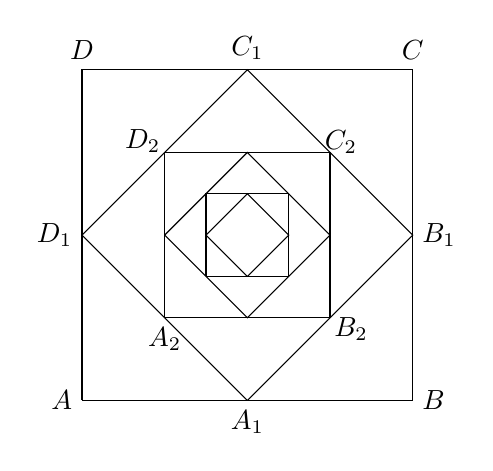
\begin{tikzpicture}[scale=.7][>=stealth, line join=round, line cap = round]
			\draw[] (0,0) -- (6,0)--(6,6)--(0,6)--(0,0);
			\draw[] (3,0) -- (6,3)--(3,6)--(0,3)--(3,0);
			\draw[] (1.5,1.5) -- (4.5,1.5)--(4.5,4.5)--(1.5,4.5)--(1.5,1.5);
			\draw[] (1.5,3) -- (3,1.5)--(4.5,3)--(3,4.5)--(1.5,3);
			\draw[] (2.25,2.25) -- (3.75,2.25)--(3.75,3.75)--(2.25,3.75)--(2.25,2.25);
			\draw[] (3,2.25) -- (3.75,3)--(3,3.75)--(2.25,3)--(3,2.25);
			\draw (0,0)node[left]{$A$} (6,0)node[right]{$B$} (6,6)node[above]{$C$} (0,6)node[above]{$D$};
			\draw (3,0)node[below]{$A_1$} (6,3)node[right]{$B_1$} (3,6)node[above]{$C_1$} (0,3)node[left]{$D_1$};
			\draw (1.5,1.5) node[below]{$A_2$} (4.4,1.3)node[right]{$B_2$} (4.7,4.3)node[above]{$C_2$} (1.6,4.7) node[left]{$D_2$};
		\end{tikzpicture}
	\end{center}
	Gọi $S_1$, $S_2$, $S_3$,...,$S_n$,... lần lượt là diện tích hình vuông $A_1B_1C_1D_1$, $A_2B_2C_2D_2$, $A_3B_3C_3D_3$,..., $A_nB_nC_nD_n$,.... Tính tổng $S_1+S_2+S_3+...+S_n+...$.	
	
\end{vd}\dongcham{25}

\subsection{BÀI TẬP TỰ LUYỆN}

\begin{bt}%[TeX hóa SGK CD]%[Dương Quang]%[1C3B1-2]
	Cho hai dãy số $(u_n), (v_n)$ với $u_n=3+\dfrac{1}{n}; v_n=5-\dfrac{2}{n^2}$. Tính các giới hạn sau:
	\begin{enumEX}{1}
		\item $\lim\limits_{n \to +\infty}u_n, \lim\limits_{n \to +\infty}v_n$.
		\item $\lim\limits_{n \to +\infty}\left(u_n+v_n\right)$, $\lim\limits_{n \to +\infty}\left(u_n-v_n\right)$, $\lim\limits_{n \to +\infty}\left(u_n\cdot v_n\right)$, $\lim\limits_{n \to +\infty}\dfrac{u_n}{v_n}$.
	\end{enumEX}
	\loigiai{
		\begin{enumerate}
			\item Ta có  \\
			$\lim\limits_{n \to +\infty}u_n=\lim\limits_{n \to +\infty}\left(3+\dfrac{1}{n}\right)=\lim\limits_{n \to +\infty}3+\lim\limits_{n \to +\infty}\left(\dfrac{1}{n}\right)=3+0=3$.\\
			$\lim\limits_{n \to +\infty}v_n=\lim\limits_{n \to +\infty}\left(5-\dfrac{2}{n^2}\right)=\lim\limits_{n \to +\infty}5-\lim\limits_{n \to +\infty}\left(\dfrac{2}{n^2}\right)=5-0=5$.\\
			\item Ta có \\
			$\lim\limits_{n \to +\infty}\left(u_n+v_n\right)=\lim\limits_{n \to +\infty}u_n+\lim\limits_{n \to +\infty}v_n=3+5=8$.\\
			$\lim\limits_{n \to +\infty}\left(u_n-v_n\right)=\lim\limits_{n \to +\infty}u_n-\lim\limits_{n \to +\infty}v_n=3-5=-2$.\\
			$\lim\limits_{n \to +\infty}\left(u_n\cdot v_n\right)=\lim\limits_{n \to +\infty}u_n\cdot \lim\limits_{n \to +\infty}v_n=3\cdot 5=15$.\\
			$\lim\limits_{n \to +\infty}\dfrac{u_n}{v_n}=\dfrac{3}{5}$.
		\end{enumerate}
	}
\end{bt} \dongcham{10}

\begin{bt}
	Tính các giới hạn sau
	\begin{tasks}(2)
		\task $\lim\limits_{n \to +\infty}\dfrac{3n+2}{2n+3}$.
		\task $\lim\limits_{n \to +\infty}\dfrac{4n^2-1}{2n^2+n}$.
		\task $\lim\limits_{n \to +\infty}\dfrac{\sqrt{n^2+2n}-3}{n+2}$.
		\task $\lim\limits_{n \to +\infty}\dfrac{\sqrt{n^2+2n}-n-1}{\sqrt{n^2+n}+n}$.
	\end{tasks}
	\loigiai{
		\begin{tasks}(1)
			\task Chia cả tử và mẫu cho $n$ có bậc lớn nhất. Ta có : $\lim\limits_{n \to +\infty}\dfrac{3n+2}{2n+3}=\lim\dfrac{3+\dfrac{2}{n}}{2+\dfrac{3}{n}}=\dfrac{3}{2}$.
			\task Tương tự: $\lim\limits_{n \to +\infty}\dfrac{4n^2-1}{2n^2+n}=\lim\limits_{n \to +\infty}\dfrac{4-\dfrac{1}{n^2}}{2+\dfrac{1}{n}}=2$.
			\task Ta có : $\lim\limits_{n \to +\infty}\dfrac{\sqrt{1+\dfrac{2}{n}}-\dfrac{3}{n}}{1+\dfrac{2}{n}}=1$.
			\task Tương tự: $\lim\limits_{n \to +\infty}\dfrac{\sqrt{1+\dfrac{2}{n}}-1-\dfrac{1}{n}}{\sqrt{1+\dfrac{1}{n}}+1}=0$.
		\end{tasks}
	}
\end{bt} \dongcham{17}	

\begin{bt}
	Tính các giới hạn sau
	\begin{tasks}(2)
		\task $\lim\limits_{n \to +\infty}\dfrac{7. 5^n-2. 7^n}{5^n-5. 7^n}$.
		\task $\lim\limits_{n \to +\infty}\dfrac{4^{n+1}+6^{n+2}}{5^n+8^n}$.
	\end{tasks}
	\loigiai{
		\begin{enumerate}[a)]
			\item Ta có : $\lim\limits_{n \to +\infty}\dfrac{7. 5^n-2. 7^n}{5^n-5. 7^n}=\lim\limits_{n \to +\infty}\dfrac{7. \dfrac{5^n}{7^n}-2}{\dfrac{5^n}{7^n}-5}=\dfrac{2}{5}$.
			\item $\lim\limits_{n \to +\infty}\dfrac{4^{n+1}+6^{n+2}}{5^n+8^n}=\lim\limits_{n \to +\infty}\dfrac{4 \cdot \left(\dfrac{1}{2}\right)^n+36\left(\dfrac{3}{4}\right)^n}{\left(\dfrac{5}{8}\right)^n+1}=0$.
		\end{enumerate}
	}
\end{bt} \dongcham{12}

\begin{bt}
	Tính các giới hạn sau
	\begin{tasks}(2)
		\task $\lim\limits_{n \to +\infty}\left( \sqrt{n^2 + 2n} - n \right) $.
		\task $\lim\limits_{n \to +\infty}\left( \sqrt{n^3 + 2n} - n^2 \right) $.
		\task 	$\lim\limits_{n \to +\infty}(\sqrt{n^2+3n+2}-n+1)$.	
		\task $\lim\limits_{n \to +\infty}(\sqrt{n^2+2n+3}-1+n)$.
	\end{tasks}
	
	\loigiai{
		\begin{tasks}(1)
			\task Ta có
			\begin{align*}
				\lim\limits_{n \to +\infty}\left( \sqrt{n^2 + 2n} - n \right) &= \lim\limits_{n \to +\infty}\dfrac{\left( \sqrt{n^2 + 2n} - n \right) \left( \sqrt{n^2 + 2n} + n \right)}{\left( \sqrt{n^2 + 2n} + n \right)} = \lim\limits_{n \to +\infty}\dfrac{(n^2 + 2n) - n^2}{\left( \sqrt{n^2 + 2n} + n \right)} \\
				&=\lim\limits_{n \to +\infty}\dfrac{2n}{n \left( \sqrt{1 + \dfrac{2}{n}} + 1 \right)} = \lim\limits_{n \to +\infty}\dfrac{2}{\sqrt{1 + \dfrac{2}{n}} + 1} \\
				&= \dfrac{2}{\sqrt{1 - 0} + 1} = 1
			\end{align*}
			\task Ta có
			$$ \lim\limits_{n \to +\infty}\left( \sqrt{n^3 + 2n} - n^2 \right) = \lim\limits_{n \to +\infty}\left[ n^2 \left( \sqrt{\dfrac{1}{n} + \dfrac{2}{n^3}} - 1 \right) \right] $$
			Mà $\lim\limits_{n \to +\infty}n^2 = +\infty $, $\lim\limits_{n \to +\infty}\left( \sqrt{\dfrac{1}{n} + \dfrac{2}{n^3}} - 1 \right) = ( \sqrt{0 + 0} - 1) = -1 < 0$ nên
			$$ \lim\limits_{n \to +\infty}\left[ n^2 \left( \sqrt{\dfrac{1}{n} + \dfrac{2}{n^3}} - 1 \right) \right] = -\infty $$
			Vậy $\lim\limits_{n \to +\infty}\left( \sqrt{n^3 + 2n} - n^2 \right) = -\infty$.
			\task \allowdisplaybreaks \begin{align*}
				\lim\limits_{n \to +\infty}(\sqrt{n^2+3n+2}-n+1)
				&=\lim\limits_{n \to +\infty}\left[\dfrac{(n^2+3n+2)-n^2}{\sqrt{n^2+3n+2}+n} +1 \right] \\
				& = \lim\limits_{n \to +\infty}\left( \dfrac{3n+2}{\sqrt{n^2+3n+2}+n} +1\right)  \\
				&=\lim\limits_{n \to +\infty}\left( \dfrac{3+\dfrac{2}{n}}{\sqrt{1+\dfrac{3}{n}+\dfrac{2}{n^2}}+1} +1\right) \\ 
				& = \dfrac{3+0}{\sqrt{1+0+0}+1} +1 = \dfrac{3}{2} +1 = \dfrac{5}{2}
			\end{align*}
			\task Ta có $$\lim\limits_{n \to +\infty}\left(\sqrt{n^2+2n+3}-1+n\right)
				=\lim\limits_{n \to +\infty}n\left(\sqrt{1+\dfrac{2}{n}+\dfrac{3}{n^2}}-\dfrac{1}{n}+1\right)$$
				Vì $\lim\limits_{n \to +\infty}n=+\infty$, $\lim\limits_{n \to +\infty}\left(\sqrt{1+\dfrac{2}{n}+\dfrac{3}{n^2}}-\dfrac{1}{n}+1\right)=\sqrt{1+0+0}-0+1=2>0$ nên
				$$\lim\limits_{n \to +\infty}n\left(\sqrt{1+\dfrac{2}{n}+\dfrac{3}{n^2}}-\dfrac{1}{n}+1\right)=+\infty$$
				Vậy $\lim\limits_{n \to +\infty}(\sqrt{n^2+2n+3}-1+n)=+\infty$.
		\end{tasks}
		
		
	}
\end{bt} \dongcham{19}

\begin{bt}
	Tính các giới hạn sau
	\begin{tasks}(2)
		\task $\lim\limits_{n \to +\infty}\dfrac{\sin{10n}+\cos{10n}}{n^2+1}$.
		\task $\lim\limits_{n \to +\infty}\dfrac{1-\sin{n\pi}}{n+1}$.
	\end{tasks}
	\loigiai{
		\begin{tasks}(1)
			\task Vì $\bigg|\dfrac{\sin{10n}+\cos{10n}}{n^2+1}\bigg|<\dfrac{\sqrt{2}}{n^2}\ \ $mà $\lim\limits_{n \to +\infty}\dfrac{\sqrt{2}}{n^2}=0\Rightarrow \lim\limits_{n \to +\infty}\dfrac{\sin{10n}+\cos{10n}}{n^2+1}=0$.
			\task Vì $\bigg|\dfrac{1-\sin{n\pi}}{n+1}\bigg|\leq\dfrac{2}{n}\ \ $mà $\lim\limits_{n \to +\infty}\dfrac{2}{n}=0\Rightarrow \lim\limits_{n \to +\infty}\dfrac{1-\sin{n\pi}}{n+1}=0$.
	\end{tasks}}
\end{bt} \dongcham{16}

\begin{bt}%[1T3B1-6]
	Tính tổng của các cấp số nhân lùi vô hạn sau
	\begin{listEX}[2]
		\item $-\dfrac{1}{2}+\dfrac{1}{4}-\dfrac{1}{8}+\cdots+\left(-\dfrac{1}{2}\right)^n+\cdots$.
		\item $\dfrac{1}{4}+\dfrac{1}{16}+\dfrac{1}{64}+\cdots+\left(\dfrac{1}{4}\right)^n+\cdots$.
	\end{listEX}
	\loigiai{
		\begin{enumerate}
			\item Tổng trên là tổng của cấp số nhân lùi vô hạn có số hạng đầu $u_1=-\dfrac{1}{2}$ và công bội $q=-\dfrac{1}{2}$ nên 
			\[-\dfrac{1}{2}+\dfrac{1}{4}-\dfrac{1}{8}+\cdots+\left(-\dfrac{1}{2}\right)^n+\cdots=\dfrac{-\dfrac{1}{2}}{1-\left(-\dfrac{1}{2}\right)}=-\dfrac{1}{3}. \]
			\item Tổng trên là tổng của cấp số nhân lùi vô hạn có số hạng đầu $u_1=\dfrac{1}{4}$ và công bội $q=\dfrac{1}{4}$ nên 
			\[\dfrac{1}{4}+\dfrac{1}{16}+\dfrac{1}{64}+\cdots+\left(\dfrac{1}{4}\right)^n+\cdots=\dfrac{\dfrac{1}{4}}{1-\dfrac{1}{4}}=\dfrac{1}{3}. \]
		\end{enumerate}
	}
\end{bt} \dongcham{17}

\begin{bt}%[1T3B1-6]
	Viết số thập phân vô hạn tuần hoàn $0{,}444\ldots$ dưới dạng một phân số.
	\loigiai{
		Ta có \[ 0{,}444\ldots=0{,}4+0{,}04+0{,}004+\ldots=0{,}4+0{,}4\cdot \dfrac{1}{10}+0{,}4\cdot \dfrac{1}{10^2}+\ldots\]
		Do đó số $0{,}444\ldots$ là tổng của cấp số nhân lùi vô hạn có số hạng đầu $u_1=0{,4}$ và công bội $q=\dfrac{1}{10}$ nên
		\[ 0{,}444\ldots=\dfrac{0{,}4}{1-\dfrac{1}{10}}=\dfrac{4}{9}. \]
	}
\end{bt} \dongcham{12}

\begin{bt}%[1T3K1-5]
	Từ tờ giấy, cắt một hình tròn bán kính $R$ (cm) như Hình $a$. Tiếp theo, cắt hai hình tròn bán kính $\dfrac{R}{2}$ rồi chồng lên hình tròn đầu tiên như Hình $b$. Tiếp theo, cắt bốn hình tròn bán  kính $\dfrac{R}{4}$ rồi chồng lên các hình trước như Hình $c$. Cứ thế tiếp tục mãi. Tính tổng diện tích của các hình tròn.
	\begin{center}
		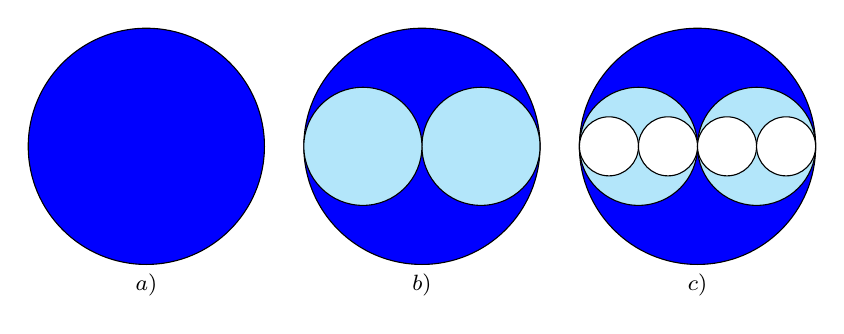
\begin{tikzpicture}[>=stealth,line join=round,line cap=round,font=\footnotesize,scale=1,declare function={r=1.5;}]
			\begin{scope}
				\draw[fill=blue] (0,0)circle(r);
				\path (0,-r) node[below]{$a)$};
			\end{scope}
			\begin{scope}[xshift={3.5cm}]
				\draw[fill=blue] (0,0)circle(r);
				\draw[fill=cyan!30] (r/2,0)circle(r/2);
				\draw[fill=cyan!30] (-r/2,0)circle(r/2);
				\path (0,-r) node[below]{$b)$};
			\end{scope}
			\begin{scope}[xshift={7cm}]
				\draw[fill=blue] (0,0)circle(r);
				\draw[fill=cyan!30] (r/2,0)circle(r/2);
				\draw[fill=cyan!30] (-r/2,0)circle(r/2);
				\foreach \i in {0,1,2,3}
				\draw[fill=white,shift={(r/2*\i,0)}] (-3*r/4,0)circle(r/4);
				\path (0,-r) node[below]{$c)$};
			\end{scope}
		\end{tikzpicture}
	\end{center}
	\loigiai{
		Diện tích của các hình tròn trong các lần cắt là
		\begin{enumerate}
			\item Lần thứ 1: $S_1=\pi R^2$.
			\item  Lần thứ 2: $S_2=2\cdot \pi \left(\dfrac{R}{2}\right)^2= \dfrac{\pi R^2}{2}$.
			\item  Lần thứ 3: $S_2=4\cdot \pi \left(\dfrac{R}{4}\right)^2= \dfrac{\pi R^2}{2^2}$.	
			\item Lần thứ $n$: $S_n= \dfrac{\pi R^2}{2^{n-1}}$.
		\end{enumerate}
		Do đó  diện tích các hình tròn lập thành một cấp số nhân lùi vô hạn có số hạng đầu $S_1=\pi R^2$ và công bội $q=\dfrac{1}{2}$ nên tổng diện tích các hình tròn là 
		\[ S_1+S_2+\cdots=\dfrac{\pi R^2}{1-\dfrac{1}{2}}=2\pi R^2. \]
	}
\end{bt} \dongcham{18}

\begin{bt} \immini{
		Cho tam giác vuông $A B C$ vuông tại $A$, có $A B=h$ và góc $B$ bằng $\alpha$ (Hình vẽ bên). Từ $A$ kẻ $A A_{1} \perp B C$, từ $A_{1}$ kẻ $A_{1} A_{2} \perp A C$, sau đó lại kẻ $A_{2} A_{3} \perp B C$. Tiếp tục quá trình trên, ta được đường gấp khúc vô hạn $A A_{1} A_{2} A_{3} \ldots$ Tính độ dài đường gấp khúc này theo $h$ và $\alpha$.}{
		
		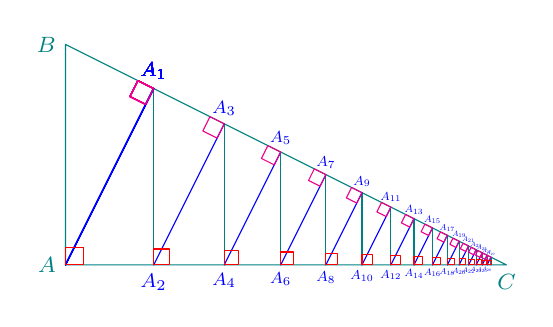
\begin{tikzpicture}[font=\footnotesize, line join=round, line cap=round, >=stealth,teal,scale=0.7]
			\def\xx{8}
			\def\yy{4}
			\pgfmathsetmacro{\gg}{90+atan(\yy/\xx)}
			\pgfmathsetmacro{\k}{(\xx)^2/((\xx)^2+(\yy)^2)}
			\tikzset{goc/.pic={
					\draw(0,0)--(0.25,0)--++(90:0.25)--++(180:0.25)--cycle;	
			}}
			\draw(0,0) node[left]{$A$}--(0,\yy)node[left]{$B$}--(\xx,0)node[below]{$C$}--cycle;
			\def\x{0}
			\foreach \i in {1,...,15}{	
				\pgfmathsetmacro{\l}{\xx-(\k)^\i*\xx}
				\draw (\l,{(\k)^\i*\yy})coordinate(A\i)--(\l,0)coordinate(B\i);
				\global \let \x =\l;	
			}
			\foreach \i in {2,...,15}{
				\pgfmathsetmacro{\a}{int(2*\i-1)}
				\pgfmathsetmacro{\b}{int(2*\i-2)}
				\pgfmathsetmacro{\j}{int(\i-1)}
				\draw[blue](A\i)node[above,scale=(0.9)^\i]{$A_{\a}$}pic[yscale=-1,rotate around ={\gg:(A\i)},scale=(0.9)^\i,magenta]{goc}--(B\j)node[below,scale=(0.9)^\j]{$A_{\b}$}pic[yscale=-1,rotate around ={-90:(B\j)},scale=(0.9)^\i,red]{goc};
				\draw[blue](A1)node[above,scale=(0.9)]{$A_{1}$}pic[yscale=-1,rotate around ={\gg:(A1)},scale=(0.9)^1,magenta]{goc}--(0,0)node[below]{}pic[yscale=-1,rotate around ={-90:(0,0)},scale=(0.9),red]{goc};
			}
		\end{tikzpicture}
			}
		\loigiai{
			\begin{itemize}
				\item Xét tam giác vuông $ABA_1$ có $AA_1=AB\cdot \sin \alpha = h\sin \alpha$.
				\item Xét tam giác vuông $AA_2A_1$ có $\widehat{BAA_1}=\widehat{AA_1A_2}$. \\
				Mặt khác $\widehat{BAA_1}+\widehat{ABC}=\widehat{AA_1A_2}+\widehat{A_1AA_2} = 180^\circ \Rightarrow \widehat{A_1AA_2} =\widehat{ABC} =\alpha$.\\
				Suy ra
				$A_1A_2=AA_1\cdot \sin \alpha = h\sin^2 \alpha$.
				\item Lập luận tương tự trên ta có $A_{n-1}A_n= h\sin^n \alpha$.
			\end{itemize}
			Như vậy $AA_1A_2A_3 \ldots = h\sin \alpha+h\sin^2 \alpha+h\sin^3\alpha+h\sin^4 \alpha \ldots $ là tổng lùi vô hạn của một cấp số nhân có số hạng đầu $u_1=h\sin \alpha$ và công bội là $\sin \alpha$. Do đó $AA_1A_2A_3 \ldots = \dfrac{h\sin \alpha}{1-\sin \alpha}$.
		}
	\end{bt} \dongcham{18}
